\documentclass[a4paper, oneside]{article}

% Packages
\usepackage{csquotes}
\usepackage{biblatex}
\addbibresource{main.bib}

\usepackage{booktabs}
\usepackage{xcolor}
\usepackage{hyperref}
\usepackage[abbreviations,symbols]{glossaries-extra}
\setabbreviationstyle{long-short}
\loadglsentries{glossary}

\usepackage{tikz}
\usepackage{amsfonts} 
\usepackage{capt-of}
\usepackage{amsmath} % or
\usepackage{mathtools}
\usepackage{pgfplots}
\usepackage{subcaption}
\usepackage{float}
\usetikzlibrary{positioning,arrows.meta}

\graphicspath{{graphics/}}
\pgfplotsset{table/search path = {data}}

% IST Colors
\definecolor{ist-cyan}{cmyk}{1,0,0,0}
\definecolor{ist-gray}{cmyk}{0.2,0,0,0.8}

% Metadata
\newcommand{\ttitle}{Cooperative Payload Transportation using Multiple Space Cobots in Microgravity Environment}
\newcommand{\tsubtitle}{}
\newcommand{\tauthor}{André Rebelo Teixeira}
\newcommand{\tdegree}{Master in Electrical and Computer Engineering}
\newcommand{\tsupervisor}{Prof. Rodrigo Martins de Matos Ventura}
\newcommand{\tdate}{November 2024}
\newcommand{\tinstitution}{Instituto Superior Técnico}

% Cover Page Command
\newcommand{\makecover}{
    \pagenumbering{gobble} % Suppress page numbering
    \begin{titlepage}
        \centering
        \includegraphics[scale=0.29]{IST_A_CMYK_POS} % Adjust to your IST logo
        \vspace{2cm}
        
        % Title
        {\LARGE\bfseries \ttitle \par}
        \vspace{0.5cm}
        {\Large \tsubtitle \par}
        \vspace{1.5cm}
        
        % Author
        {\Large \textbf{\tauthor} \par}
        \vspace{1cm}
        
        % Degree
        {\large Thesis to obtain the Master of Science Degree in \par}
        {\Large\textbf{\tdegree} \par}
        \vspace{1cm}
        
        % Supervisor
        {\large
        \begin{tabular}{rl}
            Supervisor: & \tsupervisor
        \end{tabular} \par}
        \vspace{2cm}
        
        % Institution and Date
        {\large \tinstitution \par}
        \vspace{0.5cm}
        {\large \tdate \par}
    \end{titlepage}
    \clearpage
    \pagenumbering{arabic} % Reset page numbering
}

% Document
\begin{document}

% Cover Page
\makecover

% Table of Contents
\tableofcontents
\clearpage

% Main Content
\clearpage
\section{Introduction}

\subsection{Motivation}
\par In recent years, there has been a growing interest in the use of UAVs (Unmanned Aerial Vehicles) due to their versatility and efficiency in performing a wide range of tasks. UAVs offer significant advantages by enabling faster and more effective operations, whether remotely controlled or operating autonomously using autopilot systems capable of Guidance, Navigation, and Control (GNC)~\cite{chao2010autopilots}. As discussed in detail in Section~\ref{sec:Background:Space Robots}, another emerging trend is the deployment of small-scale robots within the International Space Station (ISS). These robots, already in use, serve a variety of purposes and represent a promising direction for space exploration and operations.



Maintaining and conducting research in the ISS is not only a dangerous task, but also a rather expensive one, with the cost of 130 thousand dollars per hour of research and a limited number hours dedicated to research per year, as shown in  \href{https://www.nasa.gov/humans-in-space/commercial-and-marketing-pricing-policy/}{NASA's website}\footnote{Last accessed at 01 December 2024}, this mean that any small improvement in the efficiency of the research can lead to a large reduction in the cost, and an increase in the number of effective hours of research.

For this reason the creation of cooperative space robots capable of working both autonomously and with humans is a key factor in the future of space exploration, these robots can be used to accelerate multiple tasks, a few examples of use cases are payload transportation, autonomous inspection of the interior and exterior of the environment, and even autonomous scientific experiments. 

\subsection{Problem Definition}
Now that we know what is the main motivation behind this work, we must explain what are the main problems being tackled in this project. The most basic cooperative task a robot can do with is to be able to follow a simple trajectory outlined by a human, in this work we will be working in a higher level of control, where we try to use multiple robots to cooperatively transport a payload from point A to point B, for this to be possible, we must first create a feasible path in between these points for all the robots and the payload, this trajectory is not only a list of coordinate point, but also the acceleration and velocity desired for the robots during the movement. After this we must be able to control the robots during the trajectory, whilst keeping clear of any obstacles, both moving and static that were not known during the trajectory generation phase. 

This task needs to be divided into multiple subtasks to make it feaseble, the first one is being able to generate a feaseble trajectory for the robot's and the payload, and this implies knowing the dynamics of the robots, and the phisical parameters of the payload, such as size and mass. The second task it to be able to control the robots during the trajectory, in our case we will be using holomonic robots, this means we can have decoupled movement in all the degrees of freedom, this mean the main constraint we will have for each robot is phisical limits in acceleration, velocity and force that can be applied. The third task it to be able to detect obstacle at run time, and the the forth task is to be able to either change the original trajectory, or simply taking avoiding action is the new obstacle does not render the previous trajectory unfeaseble.

In this work we will mainly focus in steps 1, 2 and 4, and for step 3 simplification will be made, this does not mean we overlook the importance of obstacle detection in a real world scenario, simply we decided the main focus of the work should be the control and trajectory generation of the robots. The main simplification we will doing for the step 3 will be informing the robot when it comes close to obstacles and giving information such as the distance, direction and size of the robot and unoccupied space, this mean we don't need to use neither a camera nor a lidar for the detection.

For the first step we need an algorithm that is able to create a path for the robot going from point A to point B, but some constraint are needed such as, the path must be feasible, and respect the actuation limits we have for the robot, and we also must be able to generate it in a fast amount of time, otherwise the robot cannot work in a cooperative manner. For the second step, the control loop, we need to create a relieable and safe control loop that is capable of following the traectory, and since the main objective is for the controll loop to be cooperative between multiple robots, we will be working in a environment where redundancy is present, meaning less important control objectives can also be acheived, for example reduce the amount of noise generated by the robot during operation. The point 4 involves also the control loop, since it needs to be both reliable and good in path following, but also flexible enough that it can take avoiding action in real time.  



\subsection{Challenges}
\textcolor{blue}{Explain the main challenges we must tackle during the work, and how to break the problem into smaller isolated problems.}

\subsection{Objectives and Requirements}
The primary objective of this work is to enhance the current method of payload transportation within space modules. Presently, astronauts must manually move from one module to another to transport payloads, which is both time-consuming and inefficient. Our approach aims to enable fast and controlled trajectory generation, minimizing delays during valuable research hours. Additionally, the system must support cooperative operations to reduce transport time, increase payload capacity, and ensure the path followed is both safe and efficient. It is important to note that this work does not aim to address payload transportation outside a space station, as such scenarios require considerations of orbital dynamics over extended periods, as well as a robot capable of functioning in a vacuum and enduring extreme temperature variations.


\subsection{Contributions}
The contributions of this work are summarized as follows:

\begin{itemize}
    \item Development of a tunable control algorithm for multiagent systems in payload transportation within a microgravity environment. The algorithm must be able to handle the uncertainties in the system and the lack of knowledge of the payload, as well as changes in the dynamic model that can be caused by the use of different robots.  
    \item Development of a continuous trajectory planner that generates an optimal path between two points, considering system constraints, dynamic obstacles, and the uncertainty in the transported payload's properties, such as weight and distribution. 
    \item Characterization of simulation results obtained under various system architectures, focusing on the performance, efficiency, and trade-offs between centralized and decentralized approaches.
    \item Real-world testing of the cooperative algorithm using an air-bearing table.
    \item A scientific paper that details the cooperative control algorithm as well as the relation with the trajectory planning and the results obtained with this work when compared to a baseline.
    \item Creation of a GitHub Repository that houses all code and documentation necessary for testing and utilizing the materials developed throughout this work. \footnote{The repository can be accessed at https://github.com/Planning-and-Control-in-Space-Cobot.} \footnote{Please note that this work will be completed by October 31, 2025, meaning any early access to the link will not provide full content. Only open-source technologies used are currently available.}
\end{itemize}

\clearpage
\section{Background}

\subsection{Trajectory Generation}
Motion planning is a fundamental area of research, focusing on algorithms that determine how a vehicle, denoted as $\mathcal{R}$, can move optimally from a starting point $B$ to an endpoint $C$. To delve into this topic, it is essential to distinguish between \textit{path planning} and \textit{trajectory planning}. A \textbf{path} is a continous sequence of points describing how to travel from one place to another, without considering time. In contrast, a \textbf{trajectory} specifies both the path and the timing of the motion, incorporating the dynamics of the vehicle~\cite{wolek2017model}.

In~\cite{lavalle2006planning}, a mathematical framework for motion planning is presented. Here, we define the configuration space $\mathcal{C}$ as the set of all possible configurations of an agent $\mathcal{R}$ moving in an environment $\mathcal{W} = \mathbb{R}^3$ with a set of obstacles $\mathcal{O} = \{\mathcal{O}^1, \dots, \mathcal{O}^N\}$. The configuration of the agent is represented as $h = (P_t, q_t) \in SE\left(3\right)$, where $q$ denotes the orientation of the agent in quaternion form~\cite{trawny2005indirect}.

The \textbf{obstacle space}, $\mathcal{C}_{\text{obs}} \subseteq \mathcal{C}$, includes all configurations where the agent intersects with obstacles:
\[
\mathcal{C}_{\text{obs}} = \{ h \in \mathcal{C} \mid \mathcal{R}(h) \cap \mathcal{O} \neq \emptyset \}.
\]
The remaining configurations form the \textbf{free space}, $\mathcal{C}_{\text{free}} = \mathcal{C} \setminus \mathcal{C}_{\text{obs}}$, where the agent can move without collisions.

The problem becomes more complex when the robot is composed by multiple bodies. In such cases, we must avoid collisions with obstacles as well as between the robot's bodies. Instead of a single body agent, we now must consider each individual body as an agent $\{\mathcal{A}_1, \dots, \mathcal{A}_m\}$ and they specific configuration  $\{ h_1, \dots, h_m \}$. To prevent internal collisions, we define a set of collision pairs $\mathcal{P}$, where $(i, j) \in \mathcal{P}$ represents possible collisions between $\mathcal{A}_i$ and $\mathcal{A}_j$, with $i \neq j$.

The extended obstacle space accounts for both external and internal collisions:
\[
\mathcal{C}_{\text{obs}} = \left( \bigcup_{i=1}^m \{h \in \mathcal{C} \mid \mathcal{R}_i(h) \cap \mathcal{O} \neq \emptyset\} \right) \cup \left( \bigcup_{(i, j) \in \mathcal{P}} \{h \in \mathcal{C} \mid \mathcal{R}_i(h) \cap \mathcal{R}_j(h) \neq \emptyset\} \right).
\]

With this formulation, the task of motion planning is to compute a trajectory that connects the initial configuration to the goal configuration within $\mathcal{C}_{\text{free}}$.

\subsubsection{Motion Planning Algorithms}

The scheme in Figure~\ref{fig:background:trajectory generation:motion planning algorithms}, adapted from \cite{InesBatista2022Thesis}, illustrates a collection of motion planning algorithms. In this work, we focus on a few search-based methods, specifically Dijkstra’s algorithm, $A^{*}$, and $D^{*}$. Additionally, from the sampling-based group, we examine RRT and its variations, as well as PRM.

\begin{figure}[H]
    \centering
    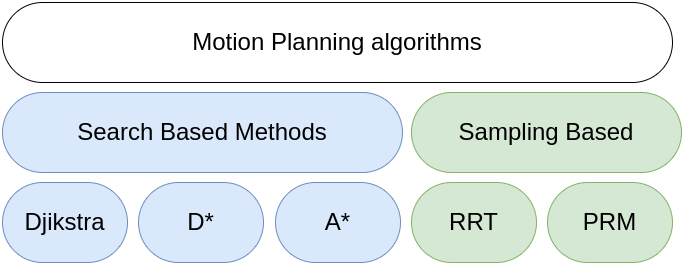
\includegraphics[width=0.7\textwidth]{Images/Background/Trajectory Generation/Motion_planing_algorithms.drawio.png}
    \caption{Scheme of motion planning algorithms~\cite{InesBatista2022Thesis}}
    \label{fig:background:trajectory generation:motion planning algorithms}
\end{figure}

\paragraph{Decomposition based Methods}

Decomposition based algorithms~\cite{latombe2012robot} partition the free configuration space $\mathcal{C}_{\text{free}}$ into a finite number of cells. From this, a connectivity graph $G = (V, E)$ is constructed, where the vertices $V$ represent the cells, and the edges $E$ denote adjacency relationships between the cells. Using this graph, standard graph search algorithms such as Dijkstra’s algorithm~\cite{dijkstra2022note}, $A^{*}$~\cite{hart1968formal}, and $D^{*}$~\cite{stentz1994optimal} can be employed to find a path.

These algorithms guarantee optimally in discrete spaces. However, the computational cost grows quadratically with the size of the search space, making them impractical for high-dimensional or complex environments where computational demands can become prohibitive.

\paragraph{Sampling-Based Methods}

Sampling-based methods~\cite{lavalle2006planning} have gained significant attention in recent years for solving motion planning problems in robotics. These methods rely on randomly sampling the configuration space $\mathcal{C}$ to build feasible paths within $\mathcal{C}_{\text{free}}$. They are generally classified into two subcategories: \textit{multiple-query} methods, which build a reusable graph for solving multiple start-goal pairs $(B, C)$, and \textit{single-query} methods, which focus on solving a single start-goal pair.

\subparagraph{Probabilistic Roadmaps (PRM)} 

PRM~\cite{kavraki1996probabilistic} is a multiple-query algorithm that constructs a roadmap starting from an empty graph $G = (N, E)$. New random configurations, $h_{\text{rand}}$, are added to the set of nodes $N$. If a collision-free path exists between $h_{\text{rand}}$ and its closest neighbors in $N$, edges are added to $E$. This process continues until a termination condition (e.g., time limit or number of configurations) is reached. The resulting graph can then be used with graph-search algorithms to solve various motion planning queries. While PRM enables exploration of large configuration spaces efficiently, it is not complete but probabilistically complete, and the solution quality depends heavily on the number of samples and neighbors considered.

\subparagraph{Rapidly-Exploring Random Trees (RRT)} 

RRT~\cite{lavalle2006planning} is a single-query algorithm that constructs a tree starting from an initial configuration. When a new sample $h_{\text{rand}}$ is generated, the algorithm attempts to connect it to the closest configuration $h_{\text{near}}$ in the tree by generating intermediate configurations ensuring a collision-free path from $h_{\text{near}}$ to $h_{\text{rand}}$. Like PRM, RRT is not complete but probabilistically complete. 

To address this, Bidirectional RRT was developed, where two trees are constructed: one growing from $B$ to $C$ and the other from $C$ to $B$. However, these algorithms are not optimal, meaning the paths found may not be the shortest. To overcome this limitation, RRT* was introduced in~\cite{karaman2011sampling}. In RRT*, new samples are connected to the nearest configuration $h_{\text{near}}$, while ensuring the minimum cost between them. Additionally, the algorithm checks whether $h_{\text{new}}$ provides a better parent-child relationship for neighboring nodes, allowing the tree to be restructured for a lower-cost solution. Though more computationally intensive, RRT* guarantees asymptotic optimality, meaning the path approaches the optimal solution as the number of samples increases.

\paragraph{Artifical potential fields} (APF)~\cite{khatib1985real}, is an approach that uses a potential field to guide the robot towards the goal while avoiding obstacles. To do this, we modelate the goals as being an atractive force, whilest making the obstacles, repulsive force. The sum of forces, the potential, is then the correct direction for the robot to move in. This method is simple and computational efficient, but it can get stuck in local minima, and it there for is not complete, to solve this problem, one can use harmonic potential functions as in \cite{kim1992real,rimon1990exact}.

In table~\ref{tab:path_planning_algorithms}, we summarize the characteristics of the path planning algorithms discussed in this section. Naturally, some algorithms can already be discarded as the computational cost is too high, this means the algorithm we are going to use latter in this work are the RRT and theirs derivations, as well as the APF method


\begin{table}[h]
    \centering
    \caption{Path planning algorithms characteristics.}
    \label{tab:path_planning_algorithms}
    \resizebox{\textwidth}{!}{%
    \begin{tabular}{lcccc}
    \hline
    \textbf{Algorithm}      & \textbf{Completeness} & \textbf{Optimality}       & \textbf{Computational Cost} & \textbf{Approach}       \\ \hline
    Search Based Methods           & complete              & optimal\textsuperscript{1} & high                        & deterministic or heuristic \\
    PRM                     & complete\textsuperscript{2} & non-optimal              & low                         & randomized             \\
    RRT                     & complete\textsuperscript{2} & non-optimal              & low                         & randomized             \\
    RRT*                    & complete\textsuperscript{2} & asymptotic optimal       & low                         & randomized             \\
    APF                     & incomplete            & optimal                   & low                         & deterministic          \\
    \end{tabular}%
    }
    
    \vspace{0.5em}
    \raggedright
    \textsuperscript{1} For discretized space.\\
    \textsuperscript{2} For infinite iterations.
\end{table}
    

\subsection{Motion Control}
In this section, we provide the necessary background from a control theory perspective to facilitate the understanding of the remainder of this work. Initially, we introduce general concepts related to optimization problems. Subsequently, we delve into the foundational principles of Nonlinear Programming (NLP), with a focus on Nonlinear Model Predictive Control (NMPC) and its application within control loops. Finally, we explore the concept of cooperative control and its relevance to multiagent systems.

\subsubsection{Optimization Problems}

An optimization problem is defined as the task of determining the best, or optimal, solution among all feasible solutions while adhering to a set of constraints. This process typically involves minimizing an objective function, often referred to as the cost function in specific applications. For cases where maximization is desired, the problem needs to be reformulated to minimize the negative of the cost function.

The general formulation of an optimization problem presented in \ref{eq:optimization_problem_with_soft_constraint}. In this formulation, \( f(x) \) represents the cost function, \( x \) denotes the decision variables, \( e_i(x) \) corresponds to equality constraints, and \( g_j(x) \) represents inequality constraints. Constraints such as \( e_i(x) = 0 \) and \( g_j(x) \geq 0 \) are referred to as hard constraints, meaning they must always be strictly satisfied. However, in certain situations, strict enforcement of constraints can render the optimization problem infeasible, especially when the constraints cannot always be satisfied due to problem-specific limitations.

To address this issue, a soft constraint term, \( sc(x) \), is introduced into the cost function. Unlike hard constraints, soft constraints do not require strict satisfaction; instead, they penalize violations within the objective function. This provides flexibility and ensures that the problem remains solvable even when some constraints cannot be strictly adhered to. The inclusion of \( sc(x) \) is particularly useful in scenarios where feasibility might otherwise be impossible with hard constraints alone.

\begin{equation}
    \begin{aligned}
        &\underset{x}{\text{minimize}} \quad f(x) + sc(x) \\
        &\text{subject to}\\
        &\quad \quad e_i(x) = 0, \quad i = 1, \dots, m, \\
        &\quad \quad \, g_j(x) \geq 0, \quad j = 1, \dots, p.
    \end{aligned}
    \label{eq:optimization_problem_with_soft_constraint}
\end{equation}

After introducing the general concept of optimization problems, Sequential Quadratic Programming (SQP) can be presented as an effective method for solving nonlinear optimization problems. SQP is particularly suitable for problems with constraints, as it approximates the original nonlinear problem by iteratively solving quadratic programming (QP) subproblems. Each subproblem optimizes a quadratic approximation of the cost function while maintaining a linearized version of the constraints.

SQP leverages second-order information about the problem, such as the Hessian of the Lagrangian, making it a powerful approach for problems requiring high accuracy. By solving the sequence of QP subproblems, SQP ensures that both the objective function and constraints are handled efficiently, even for highly nonlinear formulations.

\subsubsection{Nonlinear Model Predictive Control}

Nonlinear Model Predictive Control (NMPC) is an optimization-based technique for the feedback control of nonlinear systems, incorporating system constraints \cite{grune2017nonlinearmpc}. In order to use this technique, we need to first derive a discretized model of the system in use, since this will be necessary to predict the behavior of the system during the desired horizon. After this we solve we compute the optimal control input with relation to the chosen cost function during a certain horizon, but we use only the first control input. The optimization process is then repeated in the next time step.

As illustrated in Figure \ref{fig:simplified_mpc_control_loop}, NMPC operates as a closed-loop control system, using the current state of the system as an input. This ensures that any deviations from the system model are accounted for in subsequent iterations.

\begin{figure}[h]
    \centering
    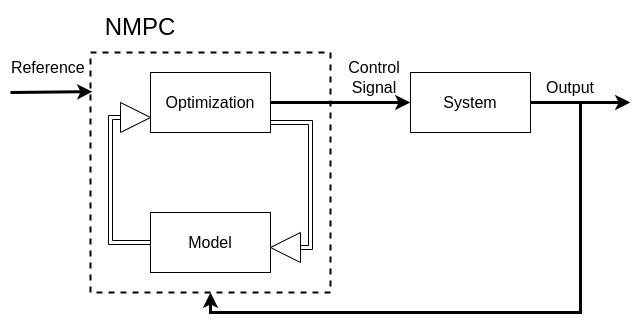
\includegraphics[width=0.8\textwidth]{Images/Background/MPC/NMPC.jpg}
    \caption{Simplified Block Diagram of an NMPC Controller}
    \label{fig:simplified_mpc_control_loop}
\end{figure}

The internal mechanism of Model Predictive Control (MPC), whether linear or nonlinear, follows the same fundamental principles~\cite{grune2017nonlinearmpc,schwenzer2021review}. 
A summary of the NMPC workflow for each time step \( t = 1, 2, \dots \) is as follows:


\begin{itemize}
    \item \textbf{State Measurement:} Measure the current state of the system, \( x(s) \in \mathbb{X} \), where \( \mathbb{X} \) is the system's state space.
    \item \textbf{Optimization Problem Definition:} We formulate the optimal control problem (OCP) as shown in \ref{eq:mpc_optimization_problem} over a horizon with dimension \( N \), where \( x(k) \) and \( u(k) \) represent the state and control signal at time \( k \) respectively. \(x_0\) represent the measured initial state of the system. The function \( f \) represents the system dynamics model, meaning with input \( x(k) \) and \( u(k) \) we compute as state at time \( k + 1 \), allowing us to predict the behavior of the system during the horizon. The function  \( l \) maps the state and control signal at time  \( k \) to a scalar value, representing the cost function we want to minimize, and \( J \) represent the cost over the full horizon. The sets \( \mathbb{X} \) and \( \mathbb{U} \) contain all the valid values for the state and control signal, respectively.
    
    \begin{equation}
        \begin{aligned}
            &\underset{u(\cdot) \in  \mathbb{U}^{N}(x_{0})}{\text{minimize}} \quad J_{N}(x_{0}, u(\cdot)) = \sum_{k=0}^{N-1} l(x(k, x_0), u(k)) \\
            &\text{subject to} \quad x(0) = x_0, \\
            &\quad \quad \quad \quad x(k+1) = f(x(k), u(k)) \\
            &\quad \quad \quad \quad x(k), \in \mathbb{X} \quad k = 0, \dots, N-1\\
            &\quad \quad \quad \quad u(k) \in \mathbb{U}, \quad k = 0, \dots, N-1.
        \end{aligned}
        \label{eq:mpc_optimization_problem}
    \end{equation}
    \item \textbf{Feedback and Update:} Use the computed NMPC feedback value \\ \( \mu_{N}(x(n)) := u(0) \) for control until the next sampling period. Remaining control values can be discarded or used as warm-start inputs for the next optimization iteration.
\end{itemize}

NMPC systems often consider two types of horizons, as discussed in \cite{schwenzer2021review}: the \textit{prediction horizon} \( N_p \), where future system dynamics are simulated, and the \textit{control horizon} \( N_c \), where optimal control inputs are computed. For simplicity, we assume \( N_c = N_p \), however in the special case that \( N_c < N_p \), the control input is held constant for the remaining steps.

\paragraph{Real time iteration scheme} first proposed in~\cite{diehl2002real}, is a common way to reduce the time taken in the controller, making it easier to run in a real time, where sometimes the max computation time is in the order of milliseconds. In this schema we compute only 1 SQP iteration per time step, and divided computation into two different phases, preparation and feedback. All operation that are not depended on the knowledge of the current state, are included in the preparation phase, since they can be executed offline, reducing the load during the online phase. The feedback phase starts when we measure the current state, we then construct the QP problem and solved it, receive as solution not the u and x, but rather us a $\Delta u$ and $\Delta x$. With this we can compute the control input as $u = u_{guess} + \Delta u$, where the $u_{guess}$ is the initial guess passed to the solver, we then apply this value for a certain time interval, during which the preparation phase is being executed as per~\cite{diehl2005real}. We then use the current $x$ and $u$ as the next iteration phase initial guess, reducing the cost of the next iteration. 

\subsubsection{Distributed NMPC}

Distributed NMPC is an extension of NMPC~\cite{muller2013distributed}, where a large complex problem is decomposed into multiple smaller subproblems that can be solved individually. Each individual controller solves its local problem while coordinating with others to ensure consensus is reached for the values of global variables. This approach is particularly useful in multiagent systems, where each agent solves its own problem while the global problem is addressed through coordination and consensus. By solving multiple smaller problems instead of one large problem, the computational burden is reduced, although the overall architecture becomes more complex. Consensus is typically achieved by computing the average of shared variables and using this new value as the start value for the next iteration, with convergence determined when the maximum difference between the variables and the average falls below a certain threshold. The Alternating Direction Method of Multipliers (ADMM)~\cite{boyd2011distributed} is commonly used to facilitate this consensus by iteratively solving local subproblems and enforcing consistency through penalty terms and dual variable updates.

\subsection{Numerical Solver}
\subsubsection{CasADi}
Normally for solving minimization problems requires the use of numerical solvers after the problem formulation phase. CasADi \cite{Andersson2019} is an open-source tool widely used for nonlinear optimization and algorithmic differentiation. In this work, CasADi is utilized due to its capability to efficiently and intuitively formulate nonlinear optimization problems, a subset of nonlinear programming problems (NLPs), using symbolic computation.

CasADi plays a central role in the implementation of the NMPC controller and the cooperative control algorithm discussed in subsequent sections. Its symbolic programming framework provides a fast and user-friendly interface for defining and solving complex optimization problems, making it an invaluable tool for this research.


\subsubsection{Initial Guess}
Given the nature of the problem at hand, it is crucial to compute the optimal solution for the robot's actuation as quickly as possible. Achieving this requires careful consideration not only of the numerical solver employed but also of the parameters used in the solver, particularly the initial values of the variables at the start of the optimization process. The performance of a solver is highly dependent on its first iteration; therefore, the initial values can significantly impact both the computation time and the likelihood of convergence. This necessitates an explanation of the concepts of cold-start and warm-start initialization.

A \textit{cold-start} refers to the case where the solver initializes the variables either randomly or using default values. In the case of CasADi, as specified in its documentation, the default initial guess is all zeros. This approach leverages no prior knowledge or potential solutions, which can lead to slower convergence or, in some cases, failure to converge. 

In contrast, a \textit{warm-start} involves providing initial values for the variables that are close to the optimal solution. This reduces computation time significantly, which is particularly advantageous when dealing with large-scale optimization problems in real-time systems, as in this work.

When employing the NMPC technique discussed earlier, the use of a warm-start is not only advantageous but straightforward to implement. This is because the optimal control problem solved at time \( t \) provides the optimal control input sequence for all times from \( t \) to \( t+N_c \), where \( N_c \) is the control horizon. Additionally, it computes the expected behavior of the system for the prediction horizon from \( t \) to \( t+N_p \), where \( N_p \) is the prediction horizon. Consequently, the solutions obtained at time \( t \) serve as an excellent initial guess for both the control inputs and the system states at time \( t+1 \). Provided the model is accurate, and the control signal applied at time \( t \) corresponds to the computed solution, the state variables and control sequence from the previous time step offer a good starting point for the new problem. In such cases, the solver only needs to make minor adjustments to account for unmodeled behaviors.

Despite the benefits of warm-starting, it is important to note that the first execution of the solver must use a cold-start, as no prior solution exists. After this initial run, the transition to a warm-start can be made seamlessly.

\subsection{Space Robotics}
Free Flyers robotics for space station environments started being tested in the ISS as early as 2006 with the SPHERES (Synchronized Position hold Engage reorient Experimental Satellites) \cite{mohan2009spheres}. This project aimed at developing an autonomous satellites servicing and in orbit manovering systems. It also helped improve docking and formation flying in a micro gravity environment. Due to the lack of a higher fidelity than the on-board global metrology, the project needed to use two perpendicular cameras to get a coarse truth sensing of the 3D operations in microgravity.

Astrobee project \cite{bualat2015astrobee} is the project that replace the SPHERES project as the free flyer project in the ISS. This project is an improvement, having more and better sensors, including, but not limited to depth cameras and color cameras, that are used in with its new mapping and planning algorithm as explained in \cite{fluckiger2018astrobee}. This new version is also equipped with a robotic arm that allows higher complex interraction with the environment. The main advantages to reseach is the creation of a fully fledge Gazebo based simulator that allows the development and testing of new algorithm here on earth with high fidelity, whilst also ahvinga all its code developed with the use of Robot Operating System (ROS) which allow for the easy integration of new code and if necessary sensors in the robot.

The Int-Ball (Internal Ball camera) project developt by the JEM \cite{mitani2019intball} was developed to move autonomously thought the inside of the ISS. This could be rather useful as a way to increase the area covered by camera in the ISS, or to use to cover a possible blind spot in the image.

The DLR developed the CIMON (Crew Interactive MObile companioN)\cite{DLR2018}, this project has multiple cameras and can be used as a mobile camera that documents the crew activities. Plan are being made to use this as a way to study human-machine interaction in a stressful environment. This robot also uses machine learning algorithm to enable speech command. 

We can see all the free flyers mentioned in the above in figure \ref{fig: BackGround: Space Robots: Free Flyers}.

\begin{figure}[H]
    \centering
    \begin{subfigure}[b]{0.45\textwidth}
        \centering
        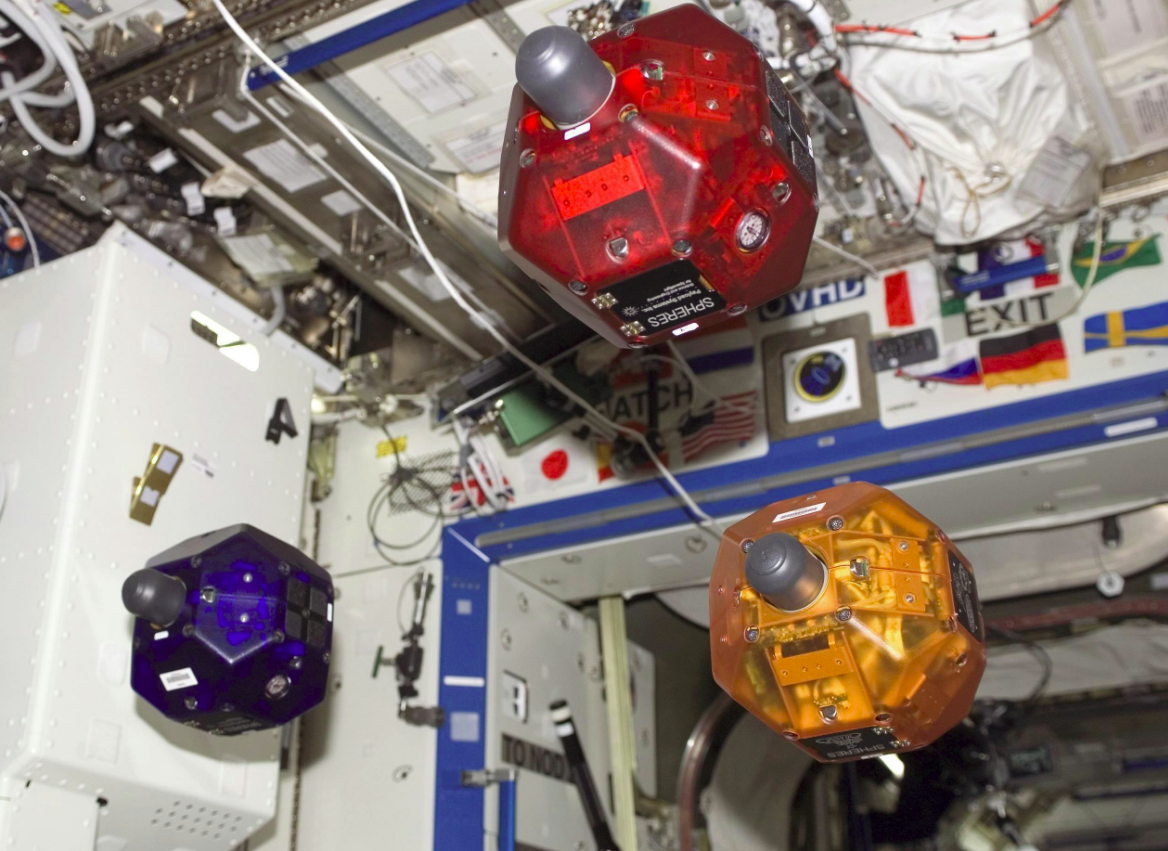
\includegraphics[width=\textwidth,height=3cm,keepaspectratio]{Images/Background/spheres.png}
        \caption{SPHERES}
        \label{fig: BackGround: Space Robots: Free Flyers: SPHERES}
    \end{subfigure}
    \hfill
    \begin{subfigure}[b]{0.45\textwidth}
        \centering
        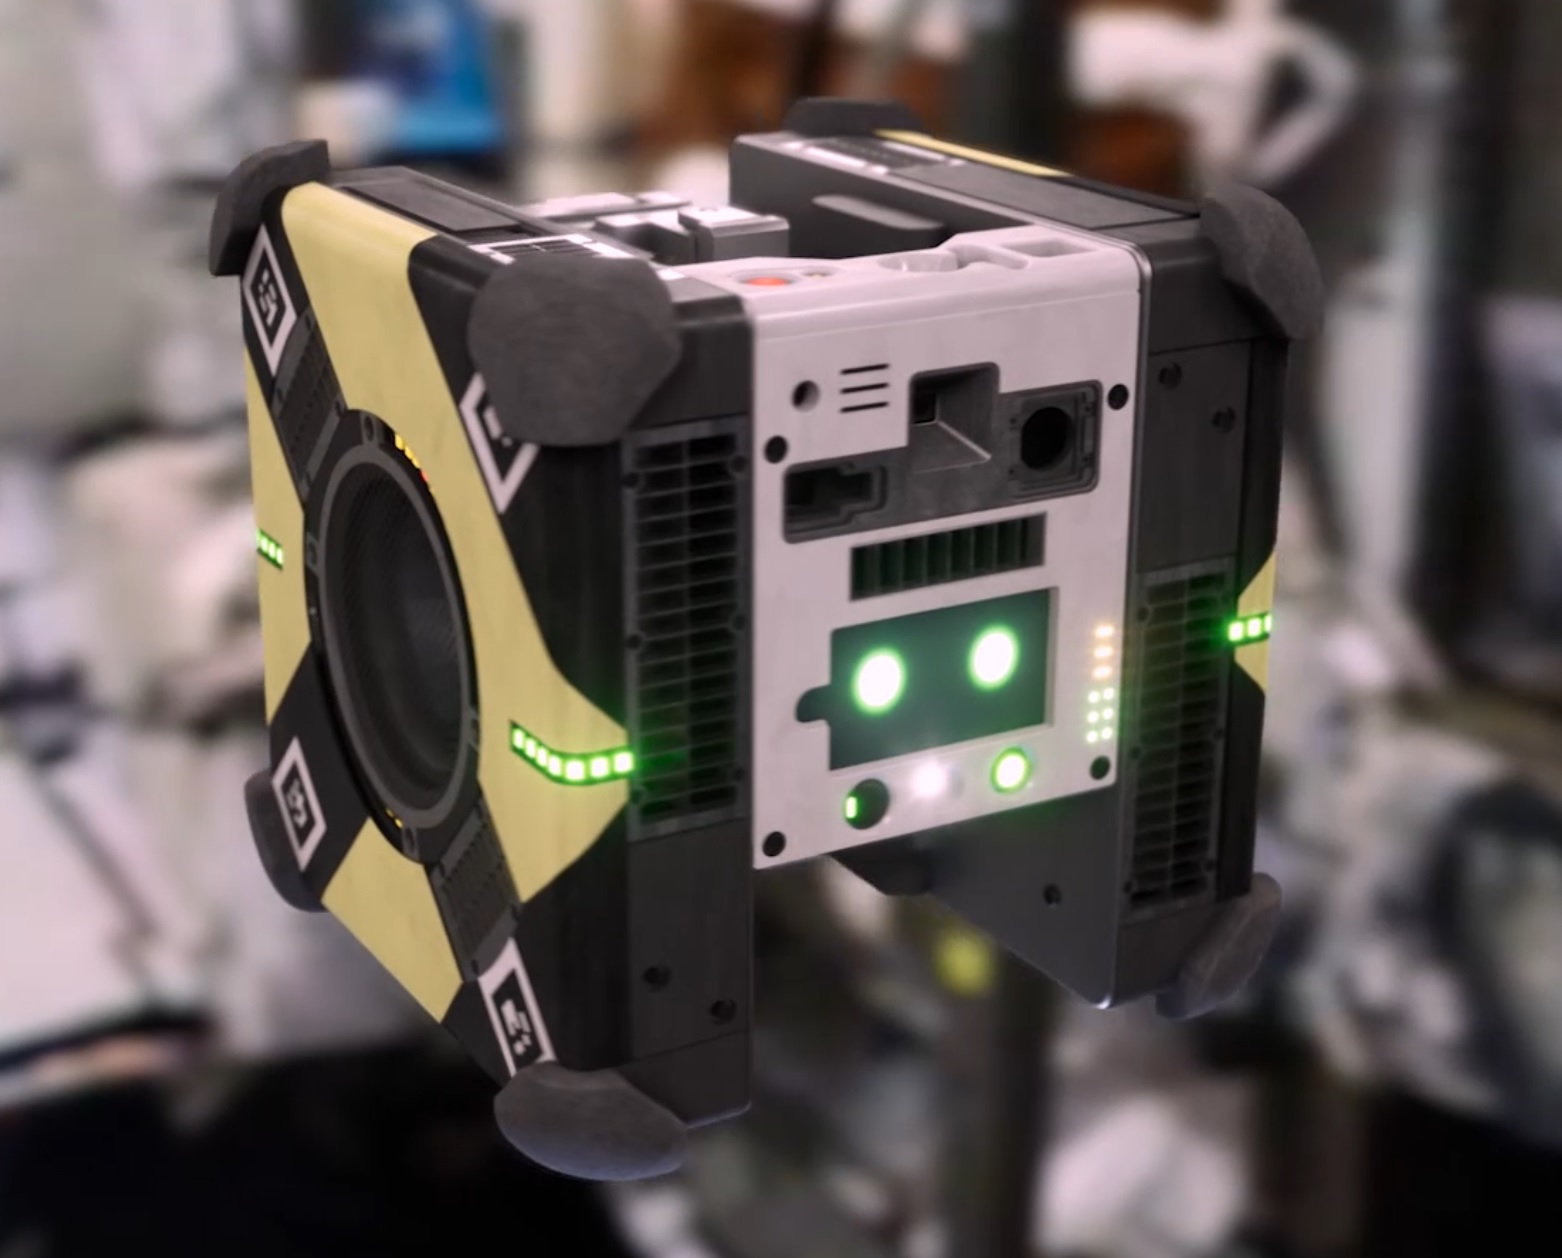
\includegraphics[width=\textwidth,height=3cm,keepaspectratio]{Images/Background/astrobee.jpg}
        \caption{Astrobee}
        \label{fig: BackGround: Space Robots: Free Flyers: Astrobee}
    \end{subfigure}
    
    \begin{subfigure}[b]{0.45\textwidth}
        \centering
        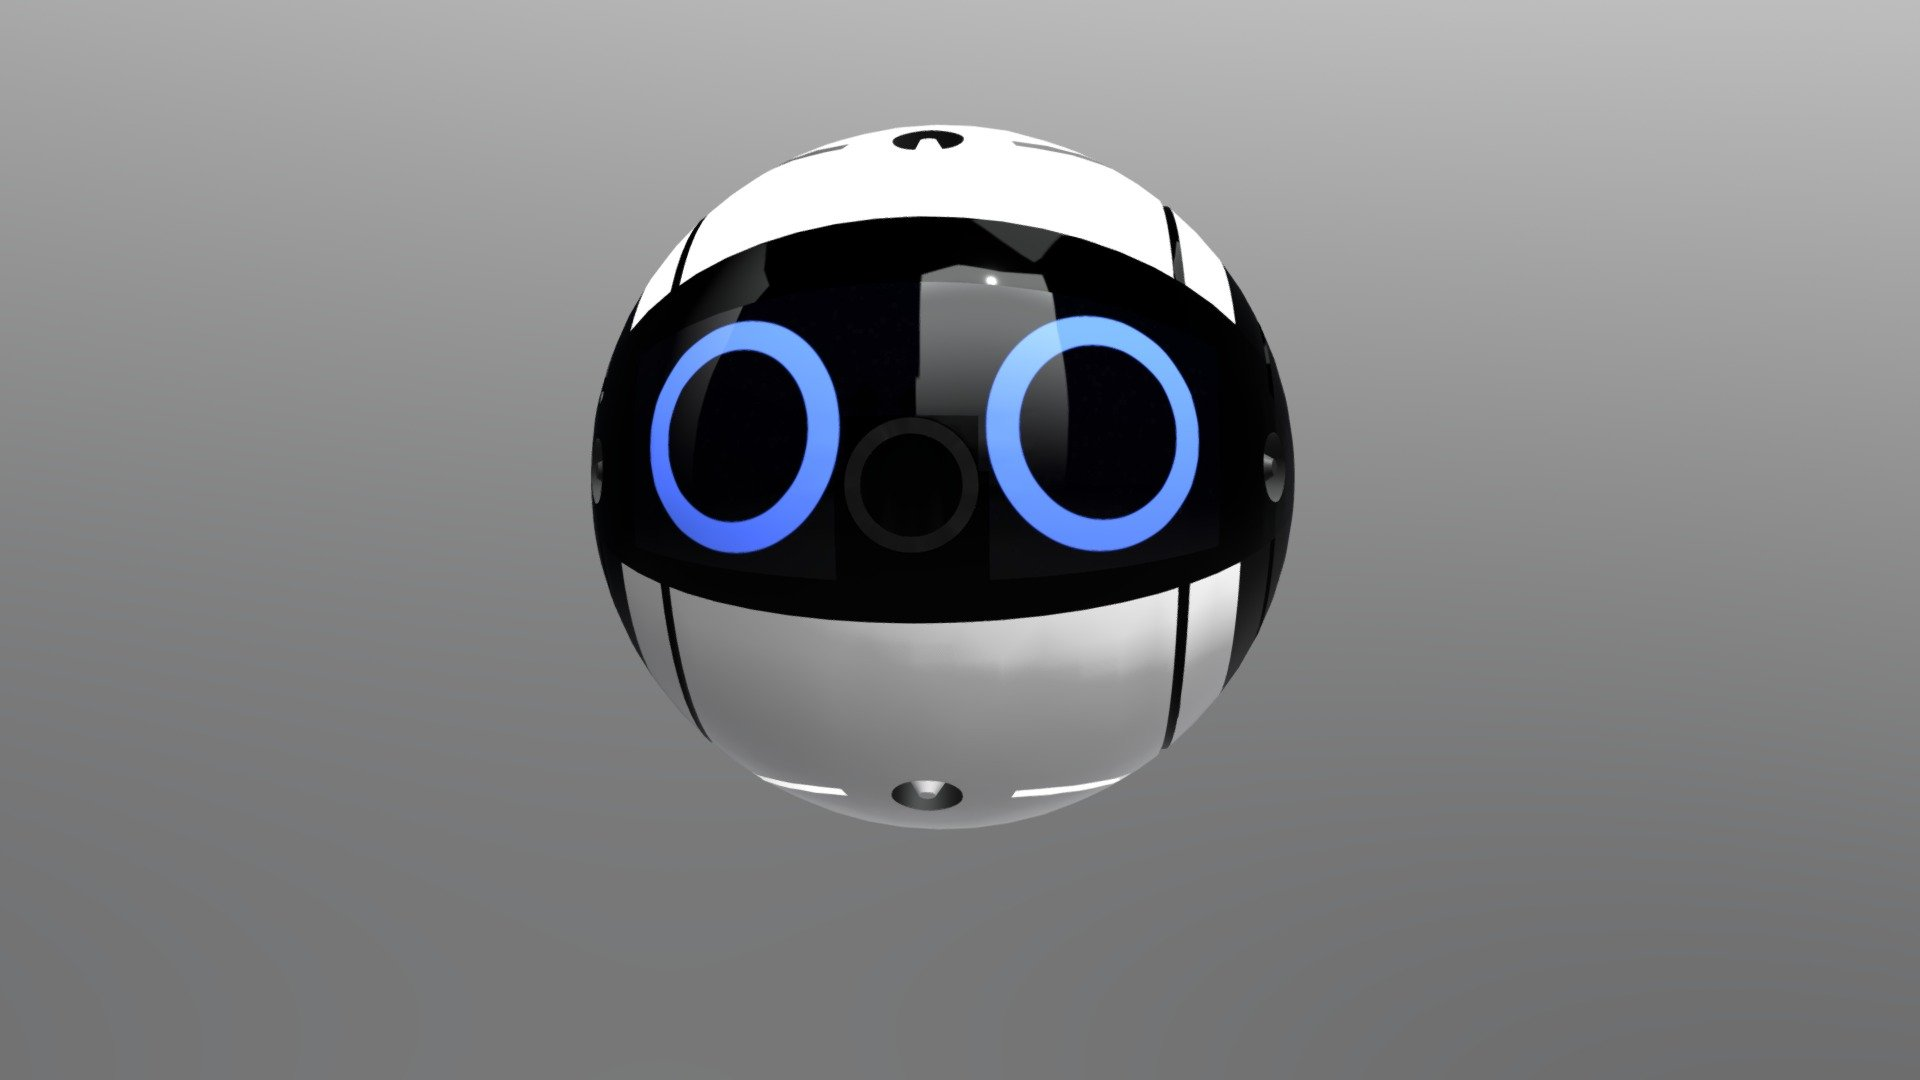
\includegraphics[width=\textwidth,height=3cm,keepaspectratio]{Images/Background/int-ball.jpeg}
        \caption{Int-Ball}
        \label{fig: BackGround: Space Robots: Free Flyers: Int-Ball}
    \end{subfigure}
    \hfill
    \begin{subfigure}[b]{0.45\textwidth}
        \centering
        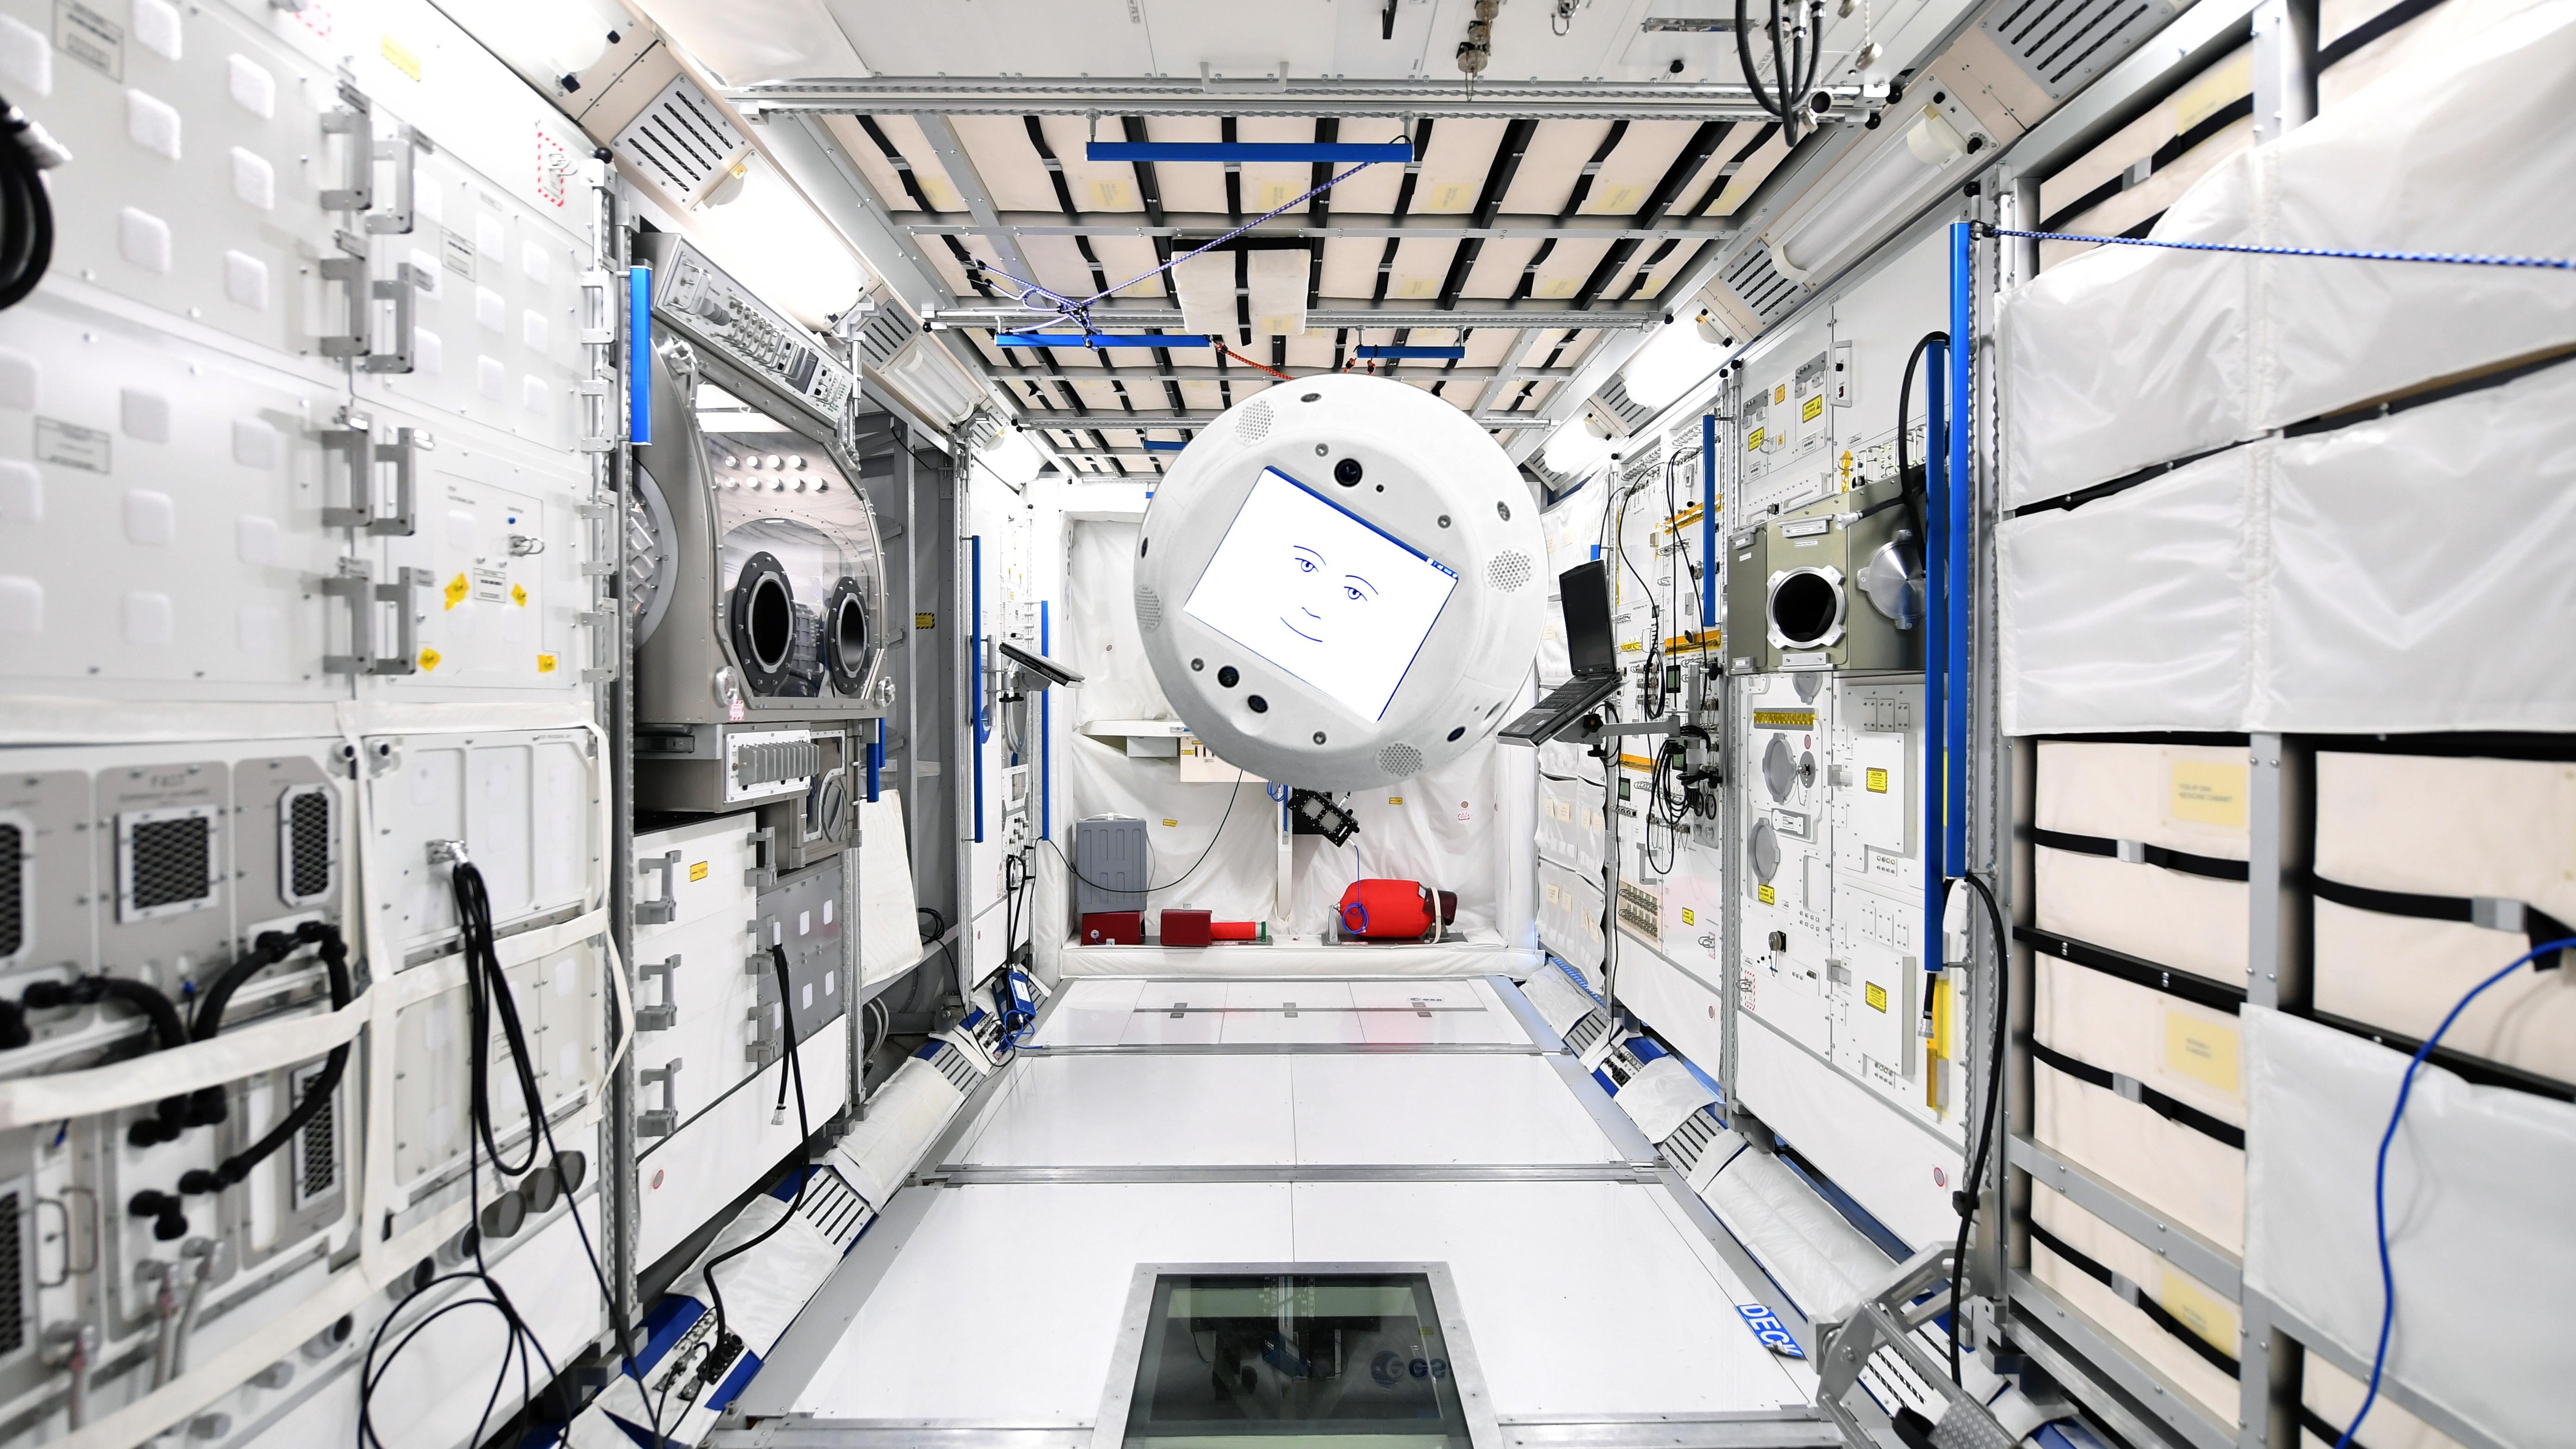
\includegraphics[width=\textwidth,height=3cm,keepaspectratio]{Images/Background/CIMON.jpeg}
        \caption{CIMON}
        \label{fig: BackGround: Space Robots: Free Flyers: CIMON}
    \end{subfigure}
    
    \caption{Free Flyers robots in the ISS}
    \label{fig: BackGround: Space Robots: Free Flyers}
\end{figure}




\clearpage
\section{State of the Art}
\textcolor{blue}{In this section, present the current state of the art for trajectory generation, optimization, cooperative payload transportation, and path-following control.}

\clearpage
\section{Proposed Approach}

\subsection{Dynamical Model}
\subsubsection{Single Robot Dynamics}
In order to be able to comprehend the dynamics of the full system, with multiple robots and payload, we must first be able to understand the dynamics of a single freeflyer in a microgravity environment. We can derive the nonlinear dynamic equations of the system in with the Newton, referencing translation, and Euler, referencing rotation, equations. This can be seen in both \cite{RoqueVentura2016spacecobot}, the main difference to this work is the use of quaternion for the representation of attitude, instead of the rotation matrix. Making the new equations be \ref{eq:Proposed approach: Motion Model: Nonlinear dynamics}, where p, is the position of the robot, v is the velocity, q is the quaternion that represents the attitude of the robot, and $\omega$ is the angular velocity of the robot, this for variables constitute the state vector of the system, x= [p, v, q, $\omega$]. The system parameters here are J $\in \mathbb{R}^{3x3}$ is the inertia matrix of the robot, and m the mass of the robot.

\begin{equation}
    \begin{cases}
        &\dot{p} = v \\
        &\dot{v} =m_i^{-1} R(q)F \\
        &\dot{q} = \frac{1}{2}Q(q) \omega \\ 
        &\dot{\omega} = J^{-1} \left(M -\omega \times J\omega \right) 
    \end{cases}
    \label{eq:Proposed approach: Motion Model: Nonlinear dynamics}
\end{equation}

The matrix R is the right-hand rotation matrix that converts from body frame to inertial frame. And the Q(q) $\in \mathbb{R}^{4x3}$ is the quaternion matrix as defined in \ref{eq:Proposed approach: Motion Model: Q matrix}

\begin{equation}
    Q\left(q\right) = 
    \begin{bmatrix}
        q_w && -q_z && q_y \\
        q_z && q_w && -q_x \\
        -q_y && q_x && q_w \\
        -q_x && -q_y && -q_z
    \end{bmatrix}
    \label{eq:Proposed approach: Motion Model: Q matrix}
\end{equation}

The vector M $\in \mathbb{R}^{3}$ is the torque applied in the robot, and F $\in \mathbb{R}^3$ is the force being applied. We can relate these to the system actuators according to \ref{eq:Proposed approach: Motion Model: Actuators}, where A is a matrix that converts from actuators space to torque and force space, and u in the actuation input vector of the system, meaning $u = \begin{bmatrix} u_{1} && \dots && u_{n} \end{bmatrix}^{T}$, where n is the number of actuators in the system and $u_{i}$ is the input of the i-th actuator. 
\begin{equation}
    \begin{pmatrix}
        F \\
        M
    \end{pmatrix} = A u
    \label{eq:Proposed approach: Motion Model: Actuators}
\end{equation}

\subsubsection{Multiple Robot Dynamics}

The dynamics presented for a single robot are not valid for the full system, since the connection between bodies also need to be taken into consideration, we can look at figure \ref{fig:Proposed Approach: Motion Model: Multi Robot System} to see a scheme of the connection.

\begin{figure}[H]
    \centering
    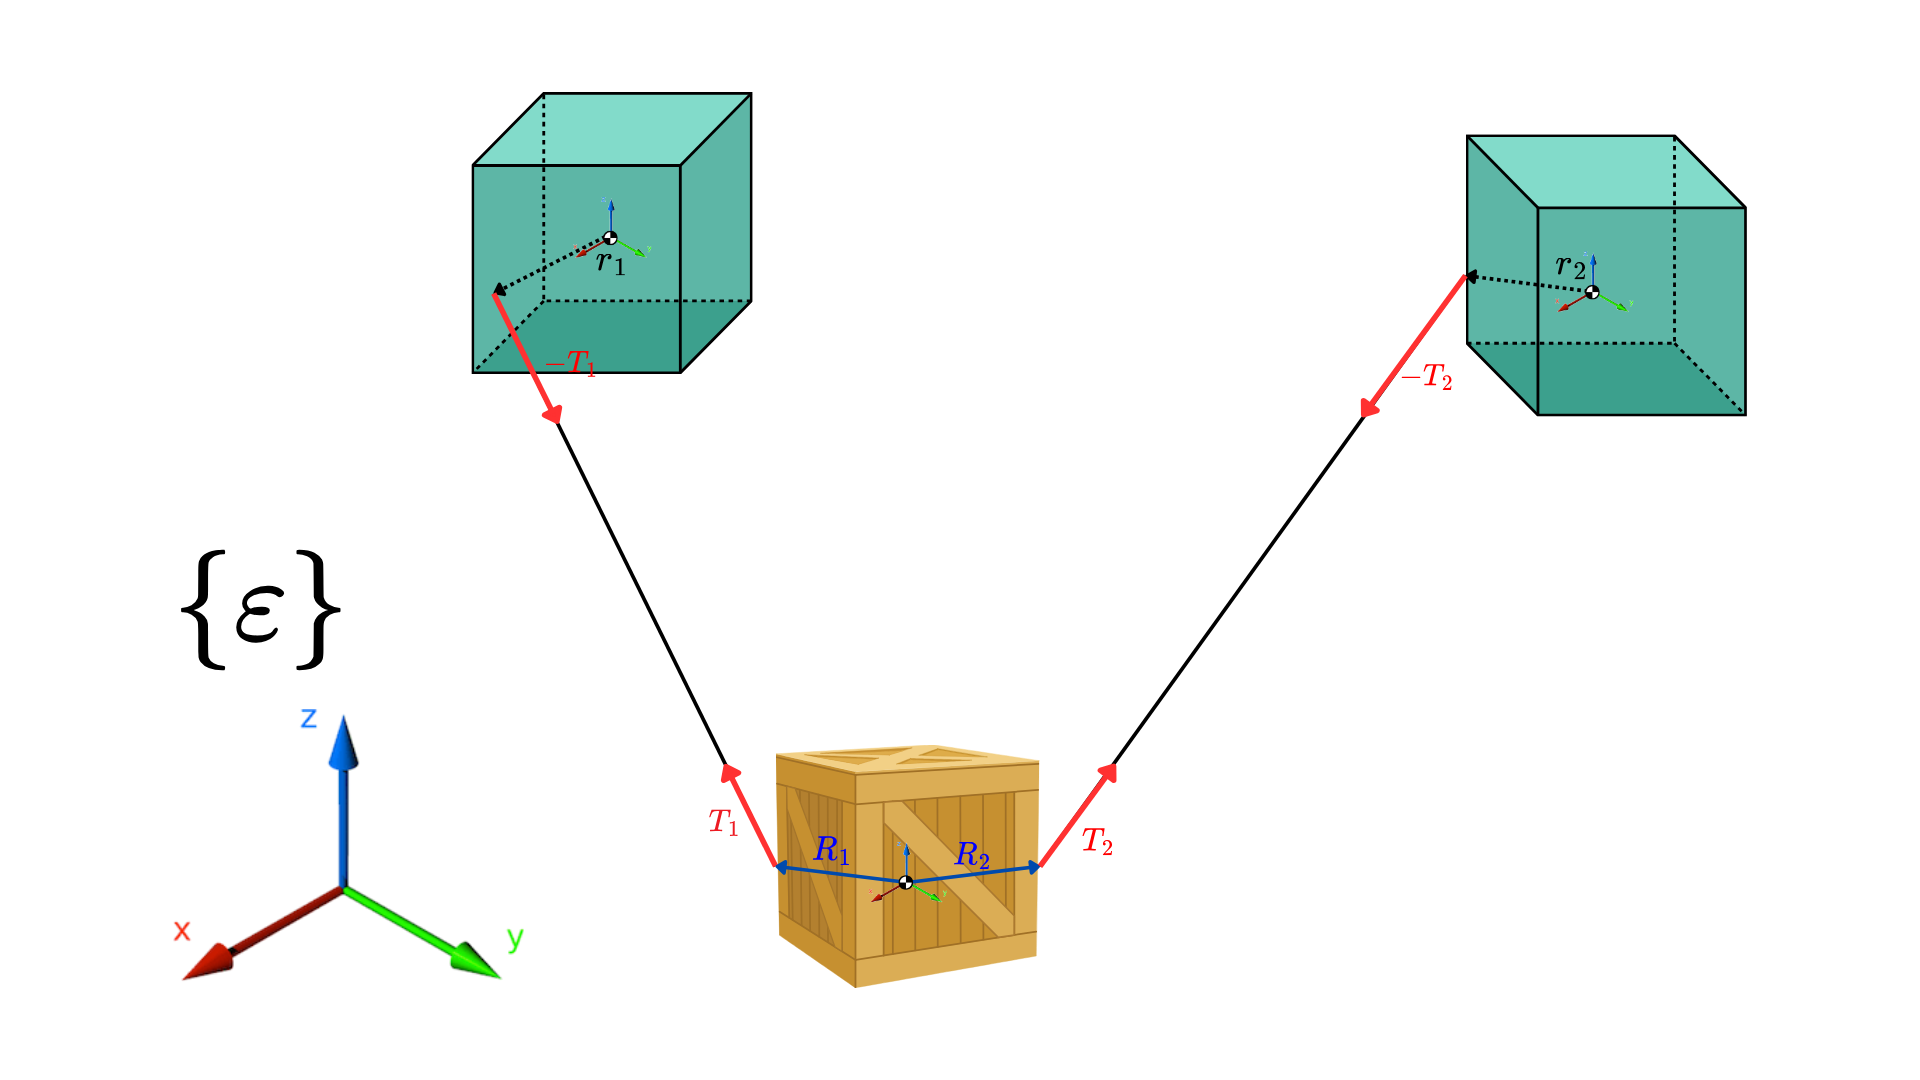
\includegraphics[width=0.7\textwidth]{Images/Propposed Aproach/multi body system.png}
    \caption{Multi Robot System}
    \label{fig:Proposed Approach: Motion Model: Multi Robot System}
\end{figure}

The dynamics of each robot in the formation will be as seen in equation \ref{eq:Proposed Approach:Motion Model: Multiple Robot Dynamics: Robot Dynamics}, where we can see the influence of the connection between the robot and the payload influence in the robot. The payload dynamics should also be considered,  we can see them in equation \ref{eq:Proposed Approach:Motion Model: Multiple Robot Dynamics: Payload Dynamics}, for both these equations the variables are defined in the following referential, $p_{i}$, $v_{i}$, $p_ {L}$, $v_{L}$, $T_{i}$ are in the inertial frame, $J_{i}$, $\omega_{i}$, $M_i$, $F_i$, $r_i$ are defined in the body frame of the i-th robot, and $J_{L}$, $\omega_{L}$, $q_L$ are defined in body frame of the payload. The matrices $R(q_{i})$ transforms from the i-th robot body frame to the inertial frame $\varepsilon$. The matrices $R(q_{i})^T$ and $R(q_{L})^T$ apply the transformation from inertial frame to the body frame of either the robot or the payload. And n in the number of robot's in the system.


\begin{equation}
    \begin{cases}
        \dot{p_i} &= v_{i} \\
        \dot{v_i} &= m_i ^{-1}(R(q_i)F_i - T_i) \\
        \dot{q_i} &= \frac{1}{2}Q(q) \omega_i \\
        \dot{\omega_i} &=J^{-1}(M_i - \omega \times J \omega - r_i \times R(q_i)^T T_i)
    \end{cases}
    \label{eq:Proposed Approach:Motion Model: Multiple Robot Dynamics: Robot Dynamics}
\end{equation}

\begin {equation}
    \begin{cases}
        \dot {p_{L}} &= v_{i} \\
        \dot {v_{L}} &= m_{i}^{-1} \sum_{i = 1}^{n} T_{i} \\
        \dot {q_{L}} &=  \frac{1}{2} Q(q) \omega_{L} \\
        \dot{\omega_{L}} &= J_{L}^{-1} (-\omega_{L} \times J_{L} \omega_{L} + \sum_{i = 1}^{n} R_{i} \times (R(q_{L})^T T_{i}))
    \end{cases}
    \label{eq:Proposed Approach:Motion Model: Multiple Robot Dynamics: Payload Dynamics}
\end{equation}

This equations are independent of the method used to connect the robot, the dynamics will be valid, using both a robotic arm, or a simpler method of using a rope to connect, the only detail ones should take into consideration from this is, if the adopted method of connection to the payload is to use a rope, then $T_i \geq 0$, since otherwise work will not be exerted in the system, this will need to be taken into consideration for the design of the controller.

\subsubsection{SpaceCobot}\label{sec:Proposed Approach: Dynamical Model: Space Cobot}

Space Cobot \cite{RoqueVentura2016spacecobot} is a holonomic, multirotor modular vehicle designed with modularity for easy maintenance and a wide range of applications. The propulsion system consists of six electric motors arranged to ensure holonomic kinematics.

Each motor in the propulsion module is 4.5 inches in size and operates independently. The configuration of these motors guarantees that the robot maintains holonomic dynamics. It is crucial to consider the bidirectional capability of the motors; although they can exert force in both directions, a slight reduction in thrust occurs when the associated propeller spins in reverse.

For a single propeller \(i\), which is rigidly linked to the robot's body frame (see Figure \ref{fig:Proposed Approach: Space Cobot: Motor graph}), both the thrust (\(F_{i}\)) and the torque (\(M_{i}\)) can be computed using the following equations. Here, \(u_i\) represents the input of the \(i\)-th actuator in rpm (rotations per second), \(K_1\) is the thrust coefficient, \(K_2\) is the torque coefficient, and \(w_i\) is either \(+1\) or \(-1\), depending on whether the propeller rotates clockwise (CW) or counterclockwise (CCW). Note that \(w_i \neq \omega\), where \(\omega\) denotes the robot's angular velocity.

\begin{figure}[H]
    \centering
    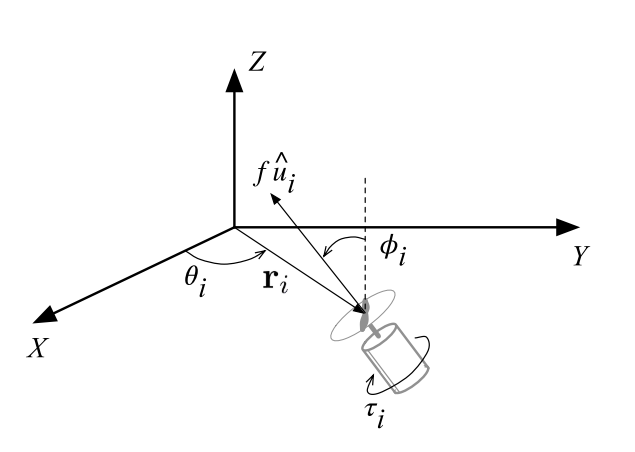
\includegraphics[width=0.7\textwidth]{Images/Propposed Aproach/space cobot motor graph.png}
    \caption{Notation used for modeling a single propeller in the Space Cobot robot. Image sourced from \cite{RoqueVentura2016spacecobot}.}
    \label{fig:Proposed Approach: Space Cobot: Motor graph}
\end{figure}

\begin{align}
    F_{i} &= f_i, & f_i &= K_{1} u_i, \\
    M_{i} &= \bar{r_{i}} \times F_{i} - \tau_{i} u_i, & \tau_{i} &= w_i K_{2} u_i
    \label{eq:Proposed Approach: Space Cobot: Motor equations}
\end{align}

The constants \(K_1\) and \(K_2\) are defined as follows (Equation \ref{eq:Proposed Approach: Space Cobot: Motor constants}), where \(\rho\) is the air density, \(D\) is the propeller diameter, and \(C_T\) and \(C_P\) are the thrust and power coefficients, respectively (dimensionless) \cite{mccormick1994aerodynamics}.

\begin{align}
    K_{1} &= \rho D^{4} C_{T}, & K_{2} &= \frac{\rho D^{5} C_{P}}{2\pi}
    \label{eq:Proposed Approach: Space Cobot: Motor constants}
\end{align}

Referring again to Figure \ref{fig:Proposed Approach: Space Cobot: Motor graph}, the position and orientation of each propeller relative to the center of mass (COM) of the robot are given by Equation \ref{eq: Proposed Approach: Space Cobot: Motor position and orientation}:

\begin{align}
    \bar{r_{i}} &= \begin{pmatrix}
        d \cos(\theta_{i}) \\ 
        d \sin(\theta_{i}) \\
        0
    \end{pmatrix}, &
    \hat{u_{i}} &= \begin{pmatrix}
        \sin(\theta_{i}) \sin(\Phi_{i}) \\
        -\cos(\theta_{i}) \sin(\Phi_{i}) \\
        \cos(\Phi_{i})
    \end{pmatrix}
    \label{eq: Proposed Approach: Space Cobot: Motor position and orientation}
\end{align}

Using general robot dynamics, we can stack the forces and moments applied to the robot and relate them to the actuation of all motors. By this logic, we derive a linear relation where:
\[
\begin{pmatrix} F_{i} \\ M_{i}  \end{pmatrix} = \hat{a_{i}} u_{i}
\]
Here, \(\hat{a_i}\) represents the actuation vector of the \(i\)-th motor, which is defined in Equation \ref{eq:Proposed Approach: Space Cobot: Actuation vector}. For the robot to maintain holonomic behavior, the configuration of the actuators must ensure that matrix \(A\) is at least rank 6. The selected configuration is shown in Table \ref{tab:Proposed Aproach: Space Cobot Motor and propeller configuration}.

\begin{equation}
\mathbf{a}_i = 
\begin{pmatrix}
K_1 \sin(\theta_i) \sin(\phi_i) \\
-K_1 \cos(\theta_i) \sin(\phi_i) \\
K_1 \cos(\phi_i) \\
[K_1 d \cos(\phi_i) - w_i K_2 \sin(\theta_i)] \sin(\phi_i) \\
-[K_1 d \cos(\phi_i) - w_i K_2 \sin(\phi_i)] \cos(\theta_i) \\
-K_1 d \sin(\phi_i) - w_i K_2 \cos(\phi_i)
\end{pmatrix}
\label{eq:Proposed Approach: Space Cobot: Actuation vector}
\end{equation}

\begin{table}[H]
\centering
\begin{tabular}{l|llllll}
Propeller (\(i\)) & 0  & 1   & 2   & 3    & 4   & 5   \\ \hline
\(\theta_{i}\)     & 0  & 60  & 120 & 180  & 240 & 300 \\
\(\Phi_{i}\)       & 55 & -55 & 55  & -55  & 55  & -55 \\
\(w_{i}\)          & -1 & 1   & -1  & 1    & -1  & 1   \\ \hline
\end{tabular}
\caption{Configuration of Propeller Placement in Space Cobot}
\label{tab:Proposed Aproach: Space Cobot Motor and propeller configuration}
\end{table}



\subsection{Trajectory Generation}

\subsection{Motion Control}
    \subsection{Simulation Environment}
\textcolor{blue}{Discuss the simulation environment used, including its advantages and limitations, such as the lack of orbital dynamics and microgravity.}

To create a realistic simulator, a physics-based simulator, Gazebo, was used. This simulator can simulate the dynamics of the system in real time, as well as the sensors employed, and it is easy to integrate with both ROS and ROS2. This integration was a key requirement, as ROS is one of the most widely used sets of libraries for robot communication. We used an already available modification of the Gazebo garden available in \href{https://github.com/DISCOWER/PX4-Space-Systems}{PX4 space system github}, this already has an easy plugin to simulate the real autopilot used, meaning all we could reuse all the code already developed in this project.

\subsection{Real-World Environment}
Even with the use of the simulator to get accurate results, it is still necessary to validate the results in real world scenario, for this we need to try and replicate the conditions of that would be found in a space station here on earth. To do this, the Space Cobot robot is fitted with both a gimbal and a base with air bearings, this allows for free rotation in a 3D space, as well as giving the robot the capability of almost frictionless movement in two different axis (XY) when in a special table. The gimbal and air bearing base can be seen in figure \ref{fig:Proposed Approach: Real World: Gimbal and Air bearing base}. With this setup, we can test the robot in a controlled environment, and compare the results against the expected results from the simulator. Some remarks should be make, with this setup, we can only test the robot in a $R^2 \times \mathbb{SO}(3)$ space, since we cannot move the robot along the Z axis, we are also subject to a pendulum effect whenever the center of mass is not aligned with the gimbal axis, and the fenomenon of guimbal lock is possible when all the rings of the guimbal are aligned, meaning we will lose one degree of freedom in the robot.

\begin{figure}[H]
    \begin{subfigure}{0.5\textwidth}
       \centering
       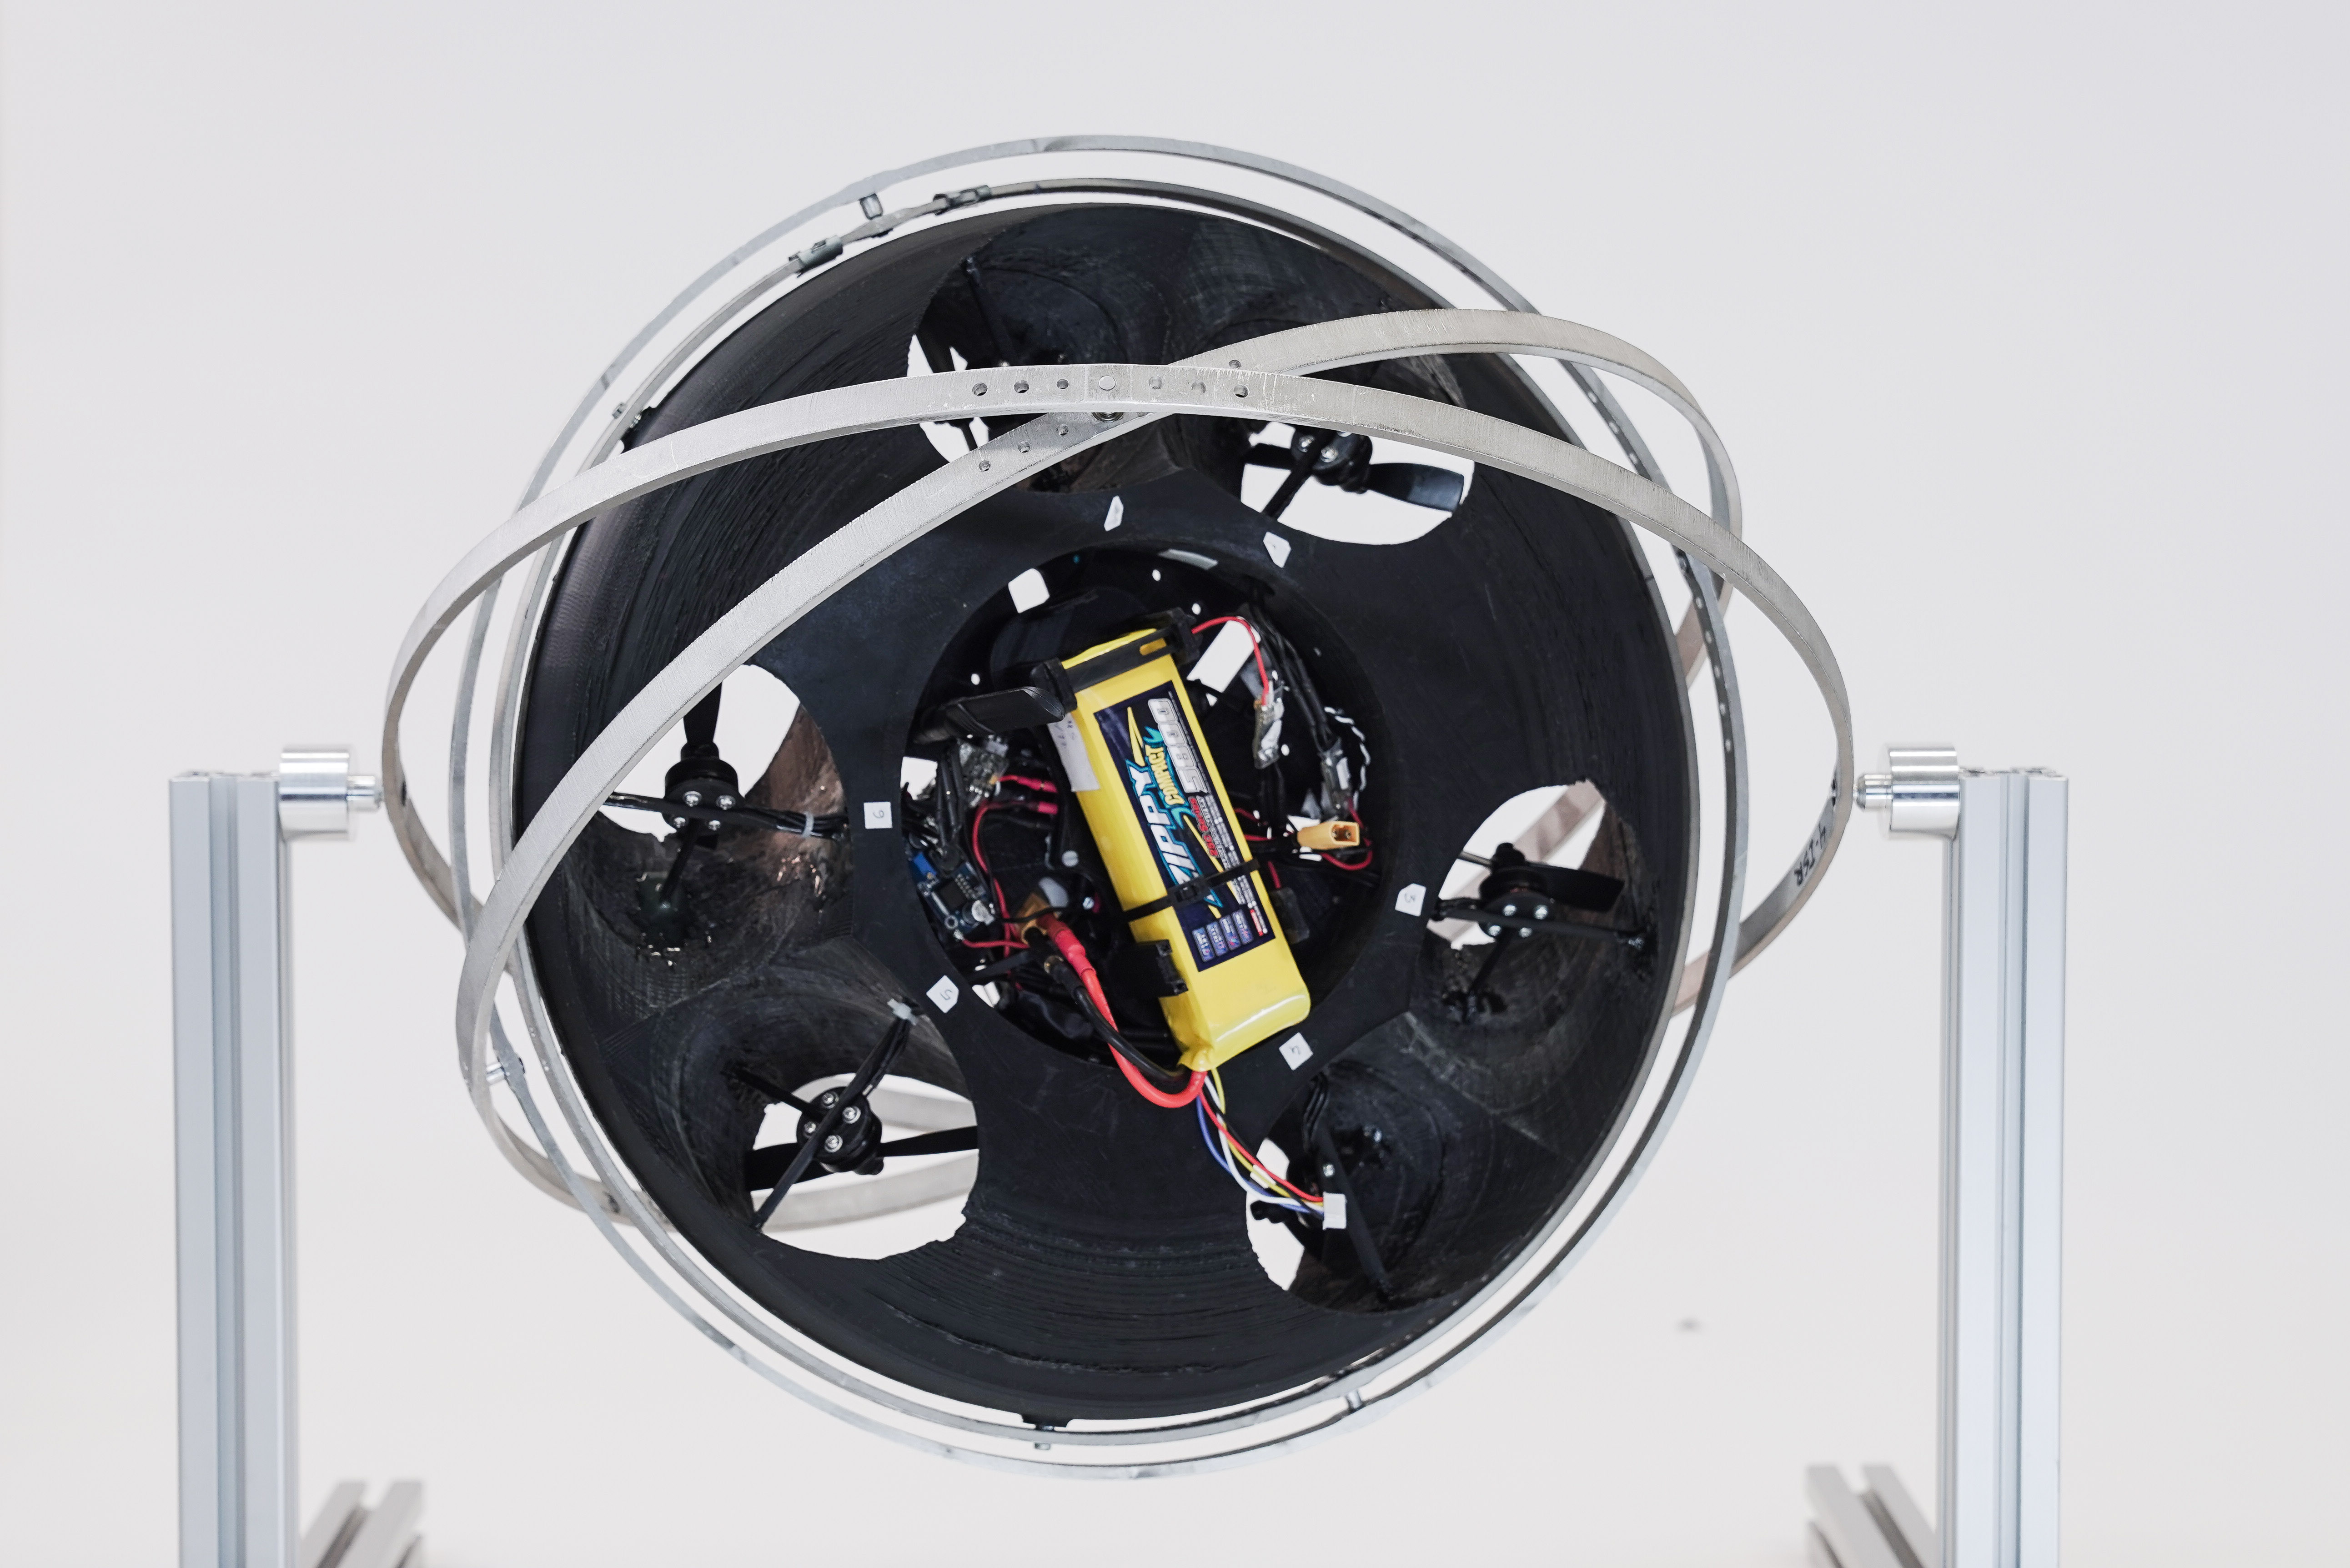
\includegraphics[width=.9\textwidth]{Images/Propposed Aproach/Gimbal.jpg} 
       \caption{Space Cobot Robot assembled inside the gimbal}
       \label{fig: Proposed Approach: Real World: Gimbal}
    \end{subfigure}
    \hfill
    \begin{subfigure}{.5\textwidth}
        \centering
        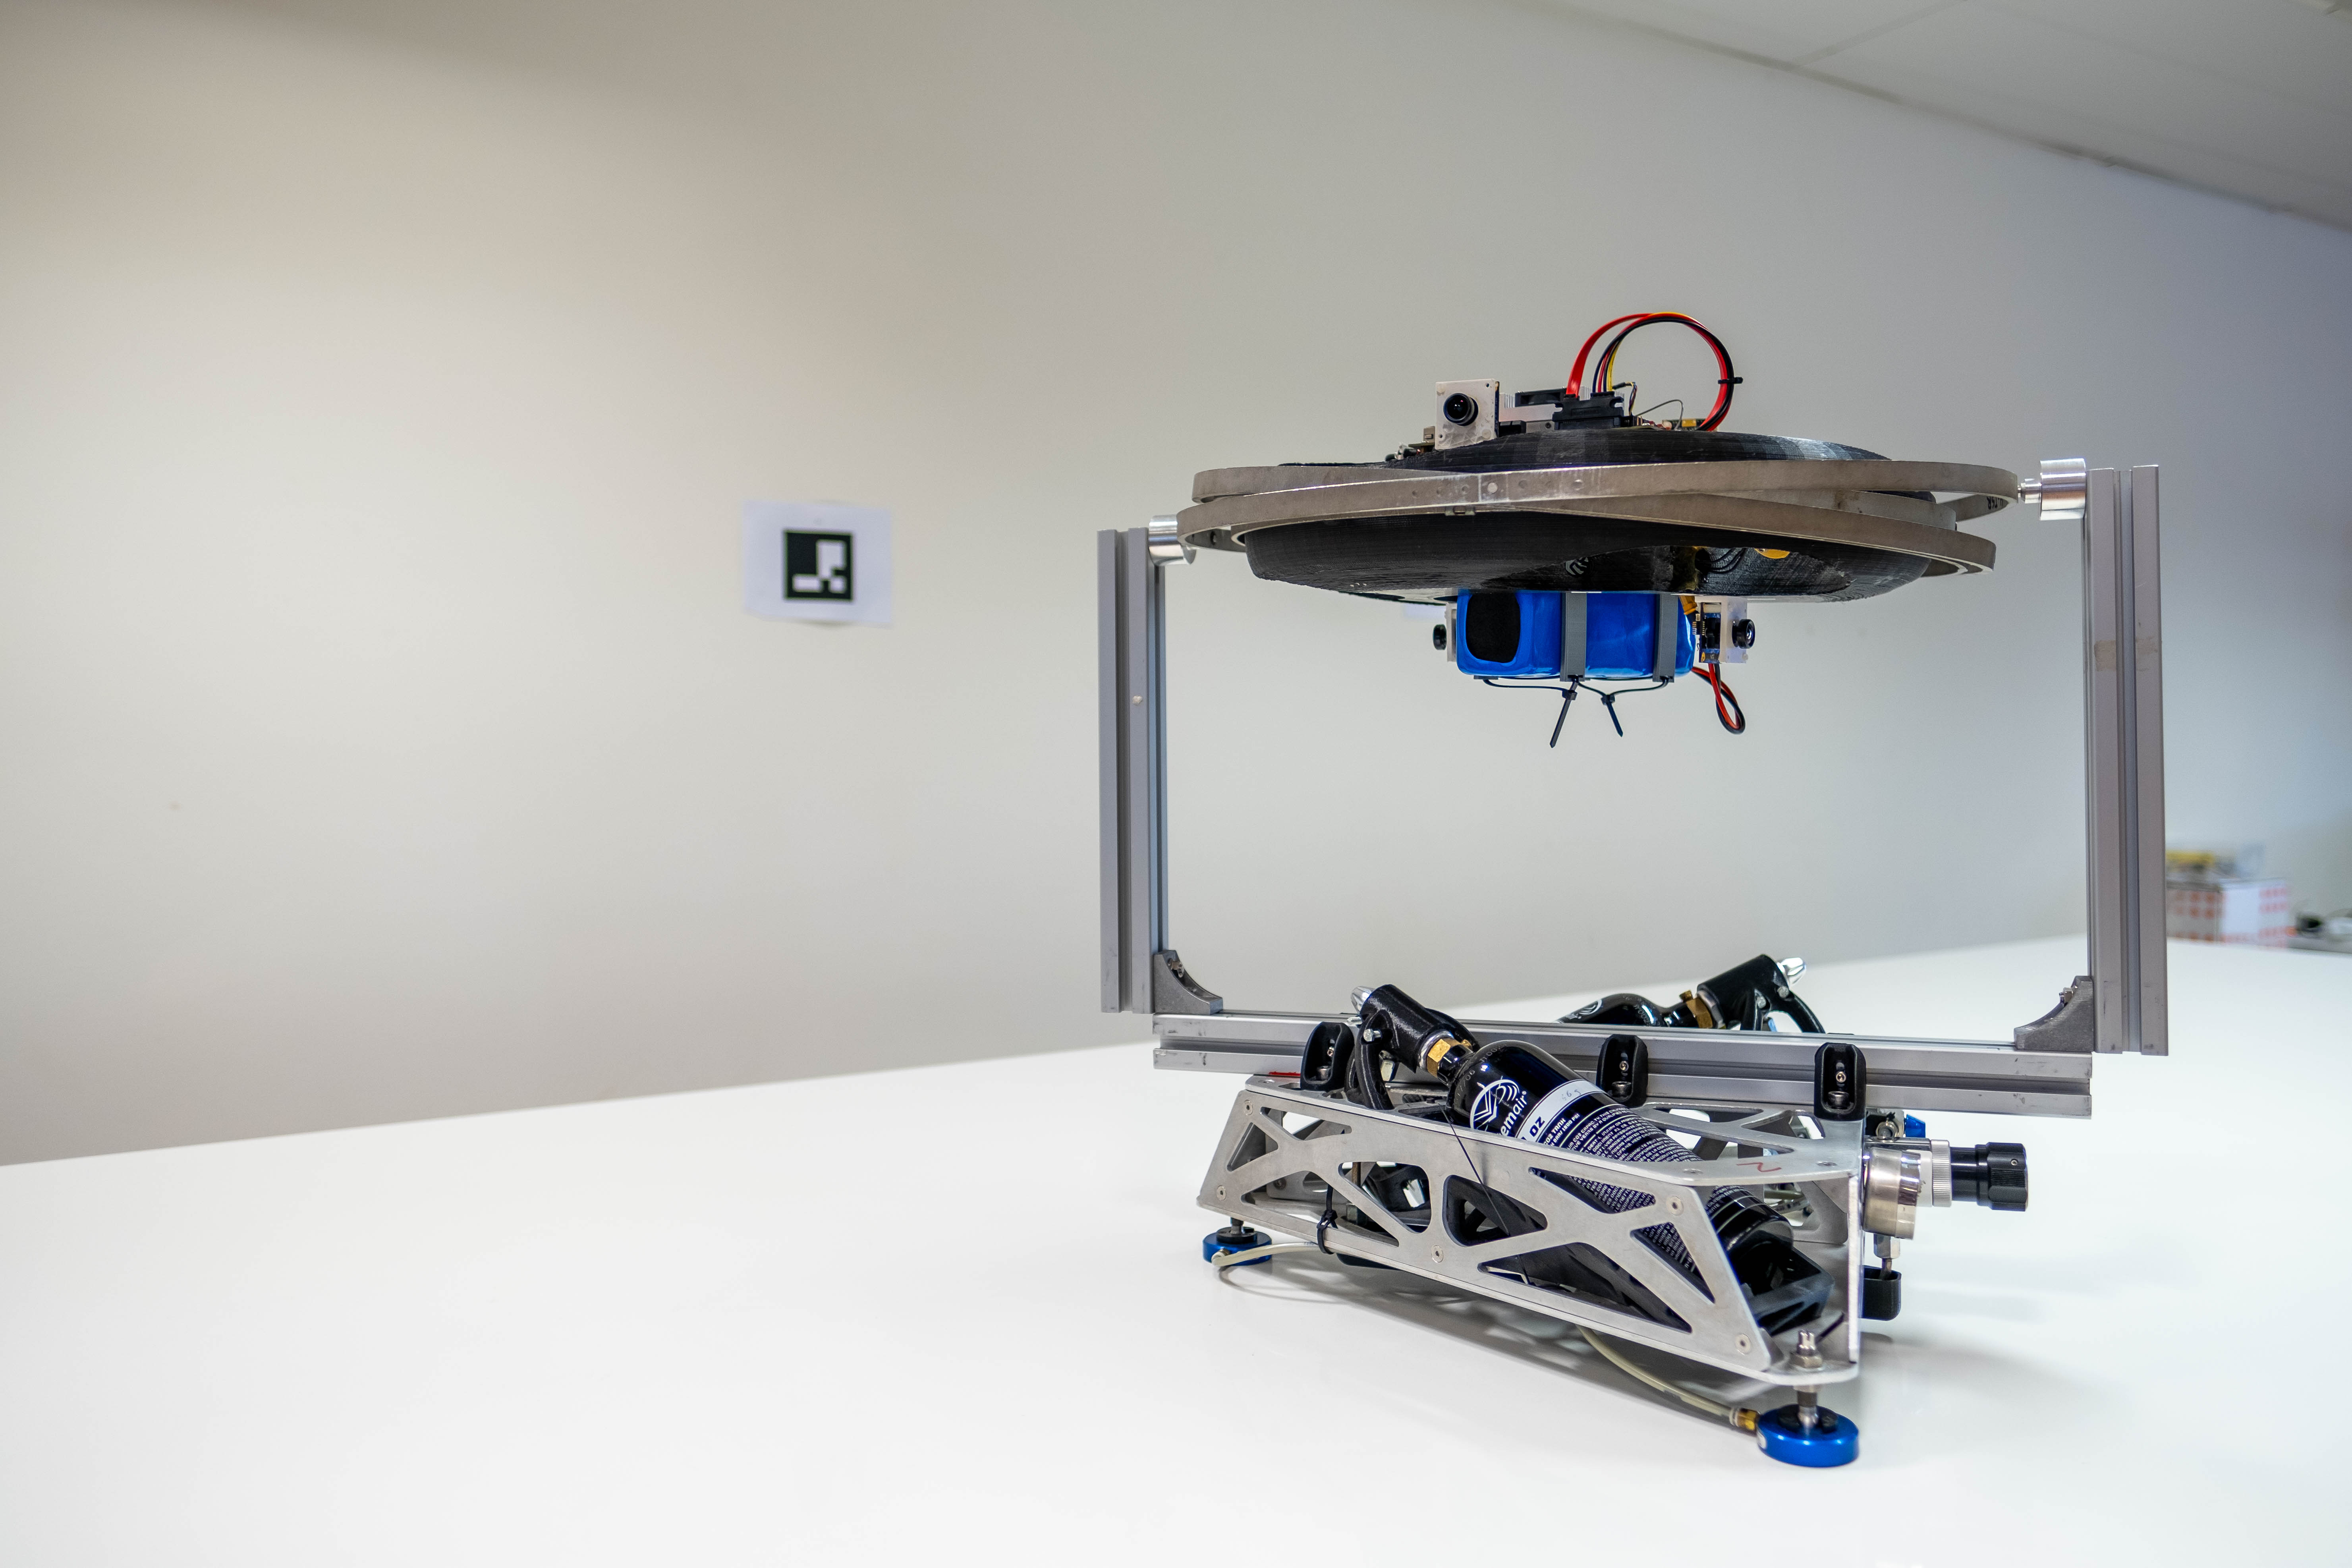
\includegraphics[width=0.9\textwidth]{Images/Propposed Aproach/Air Bearing .JPG}
        \caption{Space Cobot Robot assembled on the air bearing base}
        \label{fig: Proposed Approach: Real Word: Air Bearings}
    \end{subfigure}
    \caption{Space Cobot Robot assembled on the gimbal and air bearing base}
    \label{fig:Proposed Approach: Real World: Gimbal and Air bearing base}
\end{figure}

\clearpage
\section{Preliminary Results}

\subsection{Simulation Results}
\textcolor{blue}{Show results obtained during the project, including trajectory generation and path-following results using one and multiple robots.}

\clearpage
\section{Work Plan}
\textcolor{blue}{Explain what remains to be done for a fully functional robot, the priority of each missing step, and how to achieve them.}

% Bibliography
\nocite{*} % Include all references
\printbibliography[heading=bibintoc]

% Appendices
\appendix

\end{document}
